% !Mode:: "TeX:UTF-8"
%%  本模板推荐以下方式编译:
%%
%%     1. PDFLaTeX[推荐]
%%  注意:
%%   1. 文件默认的编码为 UTF-8 对于windows,请选用支持UTF-8编码的编辑器。
%%   2. 若是模板有什么问题,请及时与我们取得联系,Email:latexstudio@qq.com。
%%   3. 可以到  https://wenda.latexstudio.net 提问
%%   4. 请安装 最新版本的 TeXLive 地址:https://www.latexstudio.net/page/texsoftware/

\documentclass{apmcmthesis}

\usepackage{url}

%%%%%%%%%%%%填写相关信息%%%%%%%%%%%%%%%%%%%%%%%%%%
\tihao{A}                            %选题
\baominghao{2020230010136}           %报名号

\begin{document}

\pagestyle{frontmatterstyle}

\begin{abstract}
    With laser, the hatch tool of laser marking machine can be used to realize the work of making two-dimensional graphics. However, the selection and layout of hatch methods and paths greatly affect the difficulty and efficiency of incubation. The hatch problem of the laser marking machine on the two-dimensional closed graph can be equivalent to the problem of filling the two-dimensional closed curvilinear polygon with the curves connected by scattered points. Here, we provide two Python-based filling algorithms. They respectively correspond the zigzag hatch and the contour parallel hatch. Both of these two algorithms utilize vectors to the greatest extent on the basis of inward shrinking of the initial graphics to process the graphics lattice data, and use the distance between two points and the argument of vector as the basis for determining. Importantly, the algorithm automatically filters the lattice data at the sharp points of the figure after rational simplification, optimizes the shrinking of the arc with a very small radius of curvature. It also can ensure that the graphics formed after filtering can meet the requirements. This method breaks the limitation of the traditional algorithm that can only handle simple geometric figures. It provides the possibility to deal with complex curve polygons, and optimize the laser marking machine’s refined processing of complex graphics. Meanwhile, we avoid solving a large number of linear equations in the algorithm and improve its efficiency. However, because of the filtering of the lattice, the graphics we get may have some unexpected deformation. Therefore, we still need some extra program to adjust it.
    \keywords{Python\quad  filling algorithm\quad   vector\quad  zigzag hatch\quad  contour parallel hatch}
\end{abstract}



\newpage
%目录
\tableofcontents


\newpage
\pagestyle{mainmatterstyle}
\setcounter{page}{1}
\section{Introduction}
The sharpest knife, laser, has been widely used to mark specified 2D-compound curve graph. Efficiency is an important indicator for this craft. To maximize the efficiency, we need to make the hatch curves generated automatically and quickly by laser marking machine keep parallel to the boundary lines of the figures, and distribute evenly.



\subsection{Problem Restatement}
The curve used by laser etching has a certain width. In order to simplify the calculation, we approximate it to a one-dimensional curve, and set the spacing of the curve to achieve the filling effect. Taking into account the moving efficiency of the robotic arm in actual industrial production, the curve used to fill the graph must be as continuous as possible. Based on the above discussion, we can equate the problem as the optimal solution for filling a two-dimensional curve polygon with a continuous curve.


We must be clear that the zigzag hatch mentioned in the article allows the curve to be broken, but does not allow the curve to be broken at each line at the boundary, which is different from the parallel scanning hatch commonly used in the industry.


\subsection{Previous Work}
In previous work, we have learned that there has been a work of depicting a vector diagram by calculating basic data through DSP. In the processing of bitmaps, due to the large storage space occupied by bitmap files, a small amount of pixel data is selected according to the set resolution during the processing of the marking software. Such processing greatly reduces the amount of marking data of the bitmap file and improves its marking speed. Increasing the resolution of the picture can improve the fineness of the graphic marking, but due to the limitation of the scanning speed, the marking time increases accordingly.


\subsection{Problem Solving Strategies}
For the two hatching methods mentioned in the question, we originally proposed two different general algorithm. They can solve such problems universally.
For the zigzag hatch, we first indent the graphics formed by the original lattice. By finding the extreme points of the graphics, a dividing line parallel to the x-axis is made according to the traversal direction to intersect the graphics at one point. Therefore, we divide the entire graphics into a number of areas. Finally, we do zigzag hatching from top to bottom in each partition.
For the contour parallel hatch, we will iterate the steps of indentation. In the process of hatching, we will remove points that will cause overlap in the coverage area and add some points between two points far away. When the last curve generated by the iteration is about to cross, stop the iteration and partition the area formed by the last curve. Finally, we continue to iterate until reaching the filling accuracy requirement.

\section{The Description of the algorithms}


\subsection{How do we use algorithms to implement the whole process?}

The applicable objects of the algorithms in this paper are most of the two-dimensional geometric figures with curved polygons as the boundary. Both algorithms use given points data to generate appropriate point coordinate data through a certain transformation, and then connect them in a certain order to obtain the incubation path. They have a certain approximation, and through reasonable judgment conditions, the data of the generated points are appropriately screened, and points are automatically added between two points far away to complete the hatch path.



\subsubsection{The contour parallel hatch}

\begin{figure}[!ht]
    \centering
    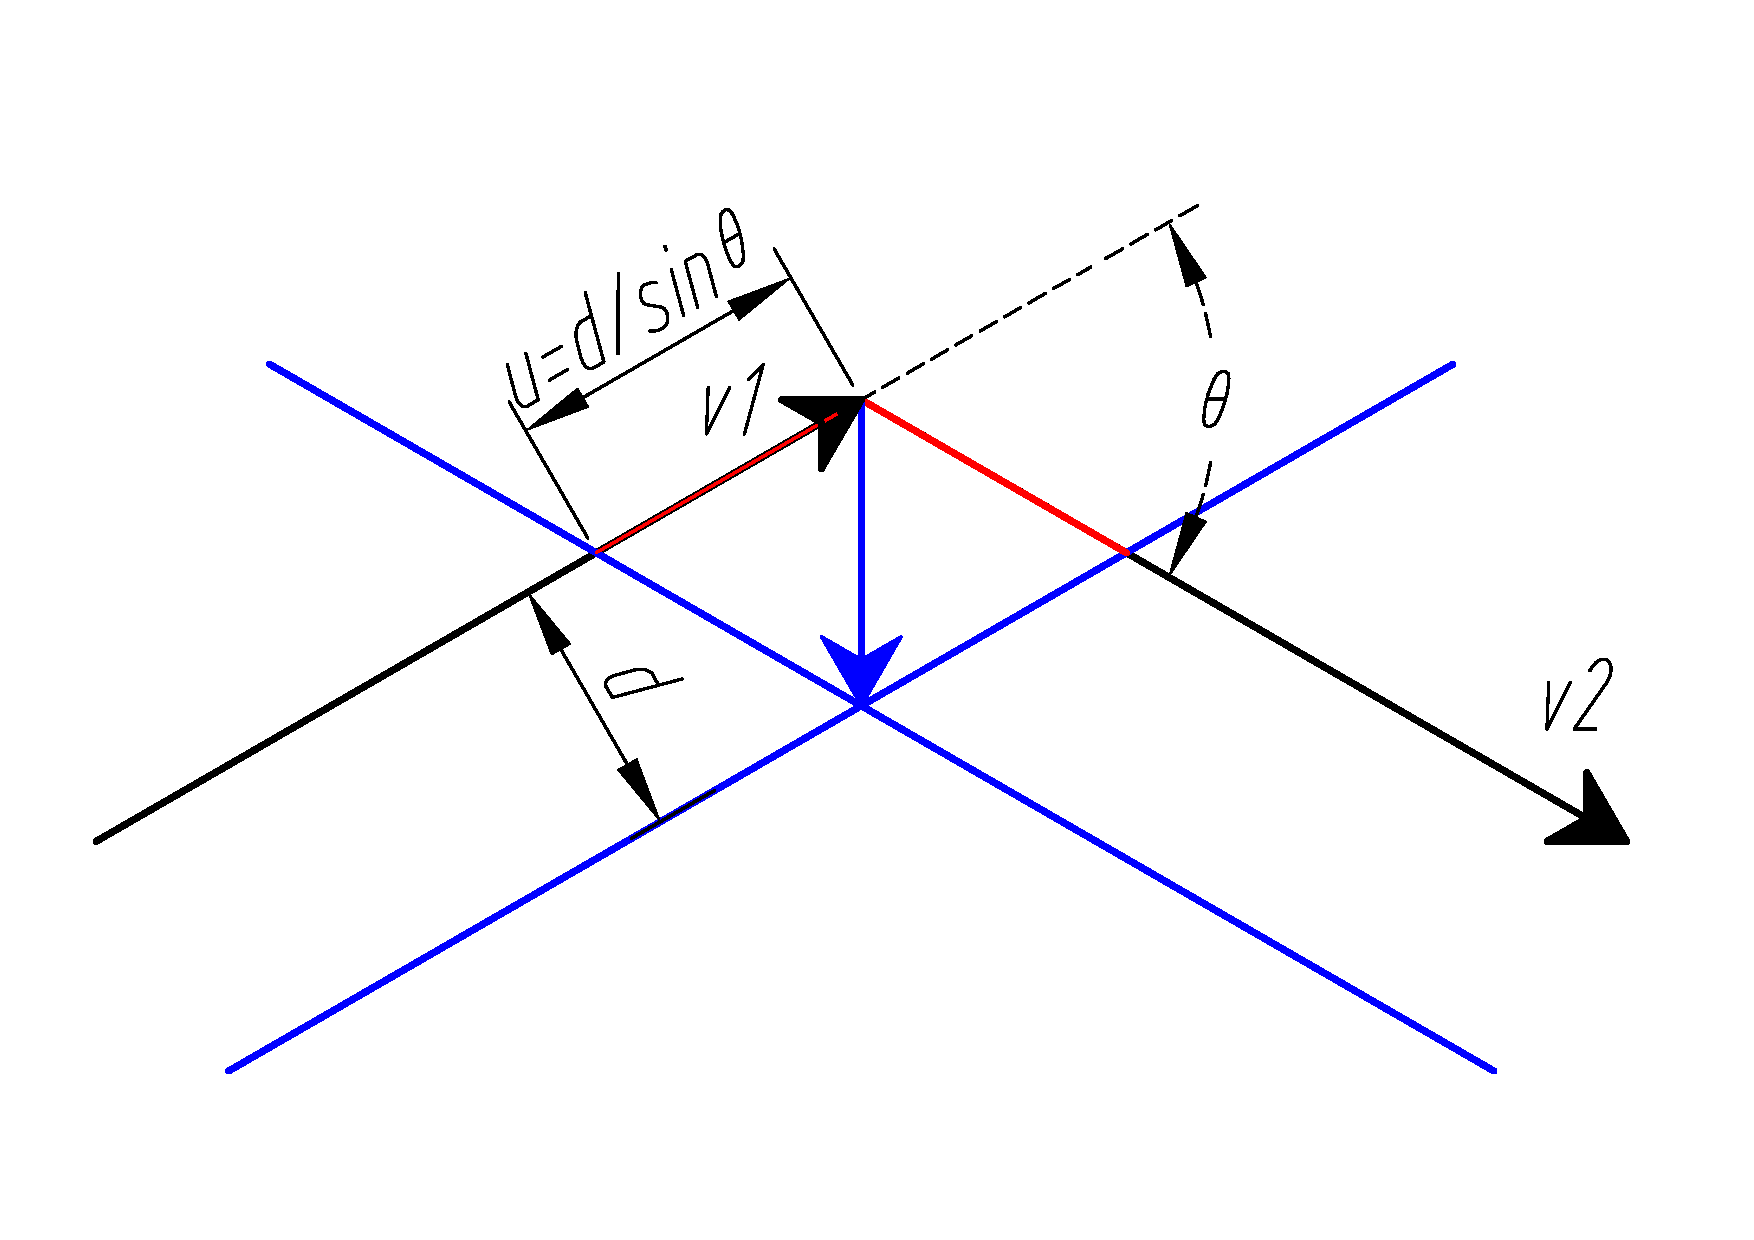
\includegraphics[width=12cm]{v}
    \caption{\CJK{UTF8}{gbsn}{The way of vector translation}}
\end{figure}

The method we use is to form two vectors through two points before and after a certain point. The straight line where the two vectors are located is translated by one precision unit into the graph, and the resulting intersection point is the mapping of the point of the new path generated inward by this point. To get the coordinates of the new point, we will unitize the vectors formed by the original three points, multiply the precision, and divide by the sine of the angle of the vector. Then we add the two vectors after processing to obtain the vector needed for transformation. The coordinates of the original point are added to the transformation vector to obtain the coordinates of the new point. According to the data given in the question, the order of the points on the outer boundary is counterclockwise. To ensure that the newly generated points are inside the original graphics, all new points must be guaranteed to be on the right side of the vector where their origin is located.


The argument and the angle between the two vectors are our basis for judgment. When this angle protrudes outside the image, the newly generated point appears inside the angle. When this angle is sunken inside the image, we add a negative sign to the transformation vector to make it inverted. Then the newly generated point appears on the outside of the angle. Through this algorithm, we can make both convex and non-convex polygons shrink inward. Performing this step in a loop, we can get the coordinate data of a new set of points. This set of data will not only be used to generate a layer of contours, but also will be used to generate the next set of lattices.


When the contour lines continue to shrink inward, the area enclosed by the contour lines gets smaller and smaller. At this time, the density of points will become larger and larger. If the distance between non-adjacent points is too small, we use these two points as the starting point and the end point, and divide the original closed figure into two closed figures, then shrink. In this way, we have completed the partitioning of the images where the contour may have multiple closed loops. Due to the limitation of the distance between two points, the circulation stops when the function can no longer generate new points.


\subsubsection{The direction parallel hatch}


Since the hatching boundary is required to have a certain distance from the graphic boundary in the title, we need to shrink the graphic using the algorithm for generating contour lines in the first step, and get a new set of point data. The horizontal lines of the zigzag hatch are arranged at equal intervals. We use the difference method to take the intersection of the boundary and the horizontal straight line whose ordinate is an integer multiple of precision, and obtain a discrete contour whose ordinate is an integer multiple of precision.


For non-convex polygons, we need to use horizontal straight lines to divide them and find the extreme points of the vertical axis in the contour sequence. If a horizontal straight line crosses this extreme point and crosses the contour on both sides of the extreme point at the same time, we take this point as the starting point of the dividing line, take the point in front of the sequence of the two intersection points as the end point, and split the contour into two closed areas. Dividing the formed areas as above, we can obtain multiple area, and do zigzag hatching in these areas.

\begin{figure}[!ht]
    \centering
    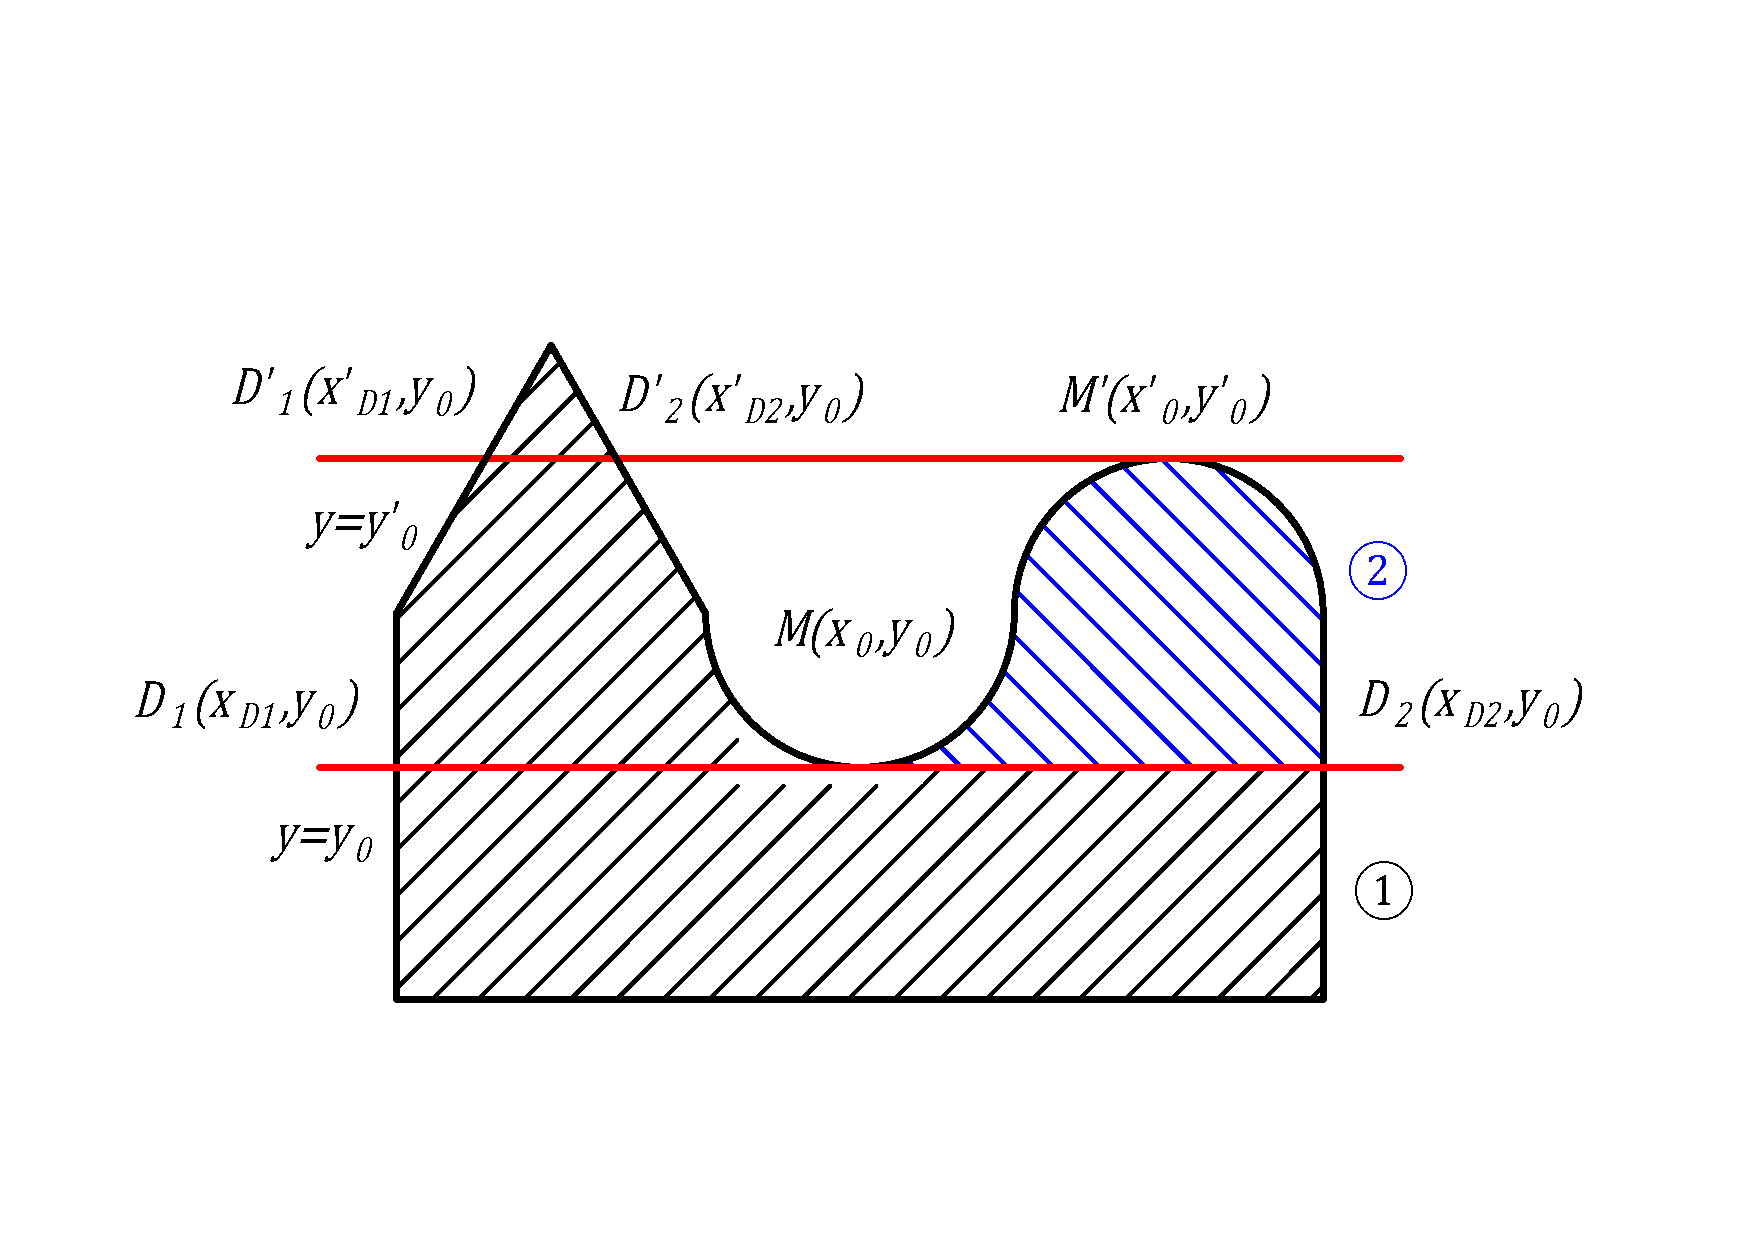
\includegraphics[width=12cm]{e}
    \caption{\CJK{UTF8}{gbsn}{Schematic diagram of segmentation method}}
\end{figure}


\subsection{The Reasonableness of approximating}


\subsubsection{Rounding of data point coordinates}
In the zigzag hatching, since the parallel lines must be parallel to the x-axis, we must make the ordinates of the data points obtained after indentation correspond to the same. This will cause deformation in the part with a smaller radius of curvature in the graph. However, due to the limitation of hatching accuracy, we have no way to fill these parts (the remaining space is not enough to make the distance between parallel lines reach the specified value), so this kind of deformation will not be reflected in hatching.

\subsubsection{Deleting and adding some special points}
In contour parallel hatch, during the iteration of the shrinking operation, we found that there are two situations that do not meet the requirements. First, the points generated after the iteration are too close to the curve before the iteration; second, the curves generated after the iteration form a closed triangle. Our algorithm will automatically identify these two situations and delete or add data points. It will cause slight deformation of the graph, for example, a smooth curve will produce some edges and corners after iteration, resulting in some small vacancies. However, when the accuracy meets the requirements, the finished product is not partially enlarged, but from the overall perspective, it is difficult to see that the indented graphics has deformed, and the existence of these vacancies cannot be seen. Moreover, the purpose of our indentation is to generate contour lines to fill the graphics, and this deformation will not interfere with our ultimate goal. So our approximation is reasonable.




\section{Operation Result}
The following is the processing result of our algorithm on the given data.

\subsection{hatch of single connected domain}


\subsubsection{The direction parallel hatch}


\begin{figure}[!ht]
    \centering
    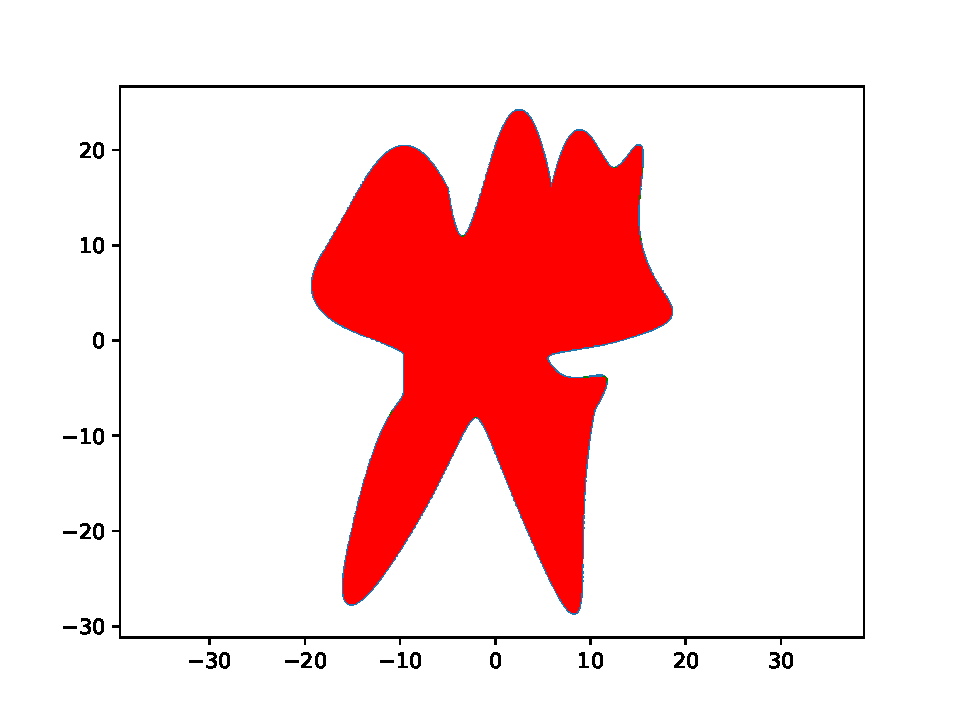
\includegraphics[width=7cm]{zigzag0.1mm} \quad 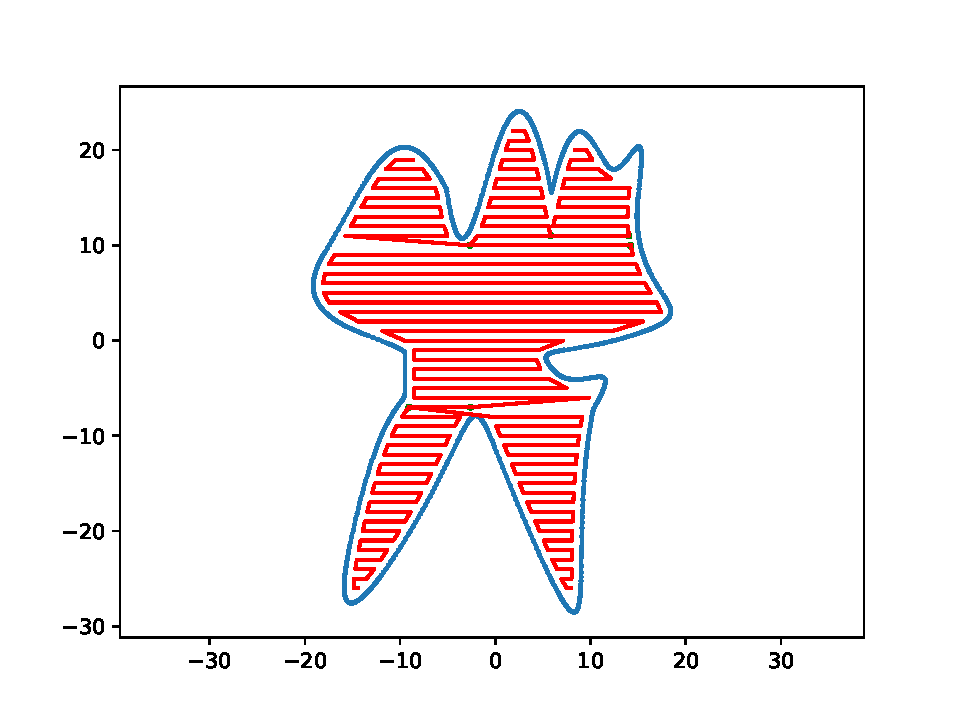
\includegraphics[width=7cm]{zigzag1mm}
    \caption{\CJK{UTF8}{gbsn}{zigzag hatching with $0.1mm$ accuracy}}
    \caption{\CJK{UTF8}{gbsn}{zigzag hatching with $1mm$ accuracy}}
\end{figure}

When the accuracy is $1mm$, the total length of the curve is $918.98mm$, the number of parallel lines is $89$, and the average elapsed time is $(6.89\times 10^3\pm 30)$ mm. When the accuracy is 0.1mm, the total length of the curve is $10022.71mm$, the number of parallel lines is $911$, and the average elapsed time is $(7.75\times 10^3\pm 40) mm$. The time-consuming ratio in the two cases is $1.12$.


It can be clearly seen from the data that after the accuracy is improved, the time-consuming increase of this algorithm is small.

\begin{figure}[!ht]
    \centering
    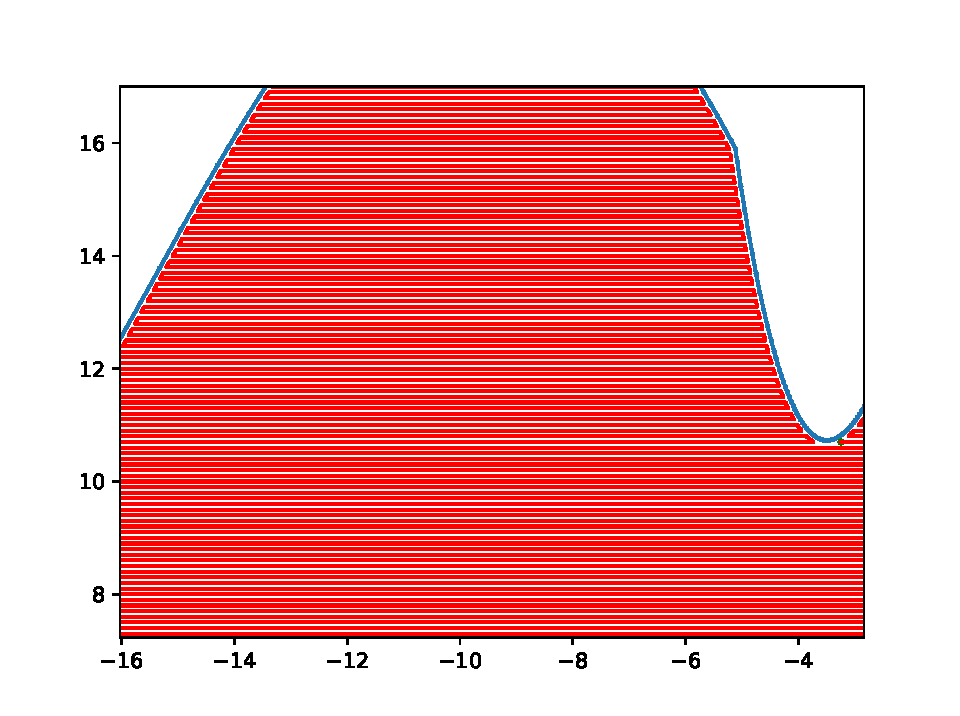
\includegraphics[width=7cm]{zigzag detail 0.1mm} \quad 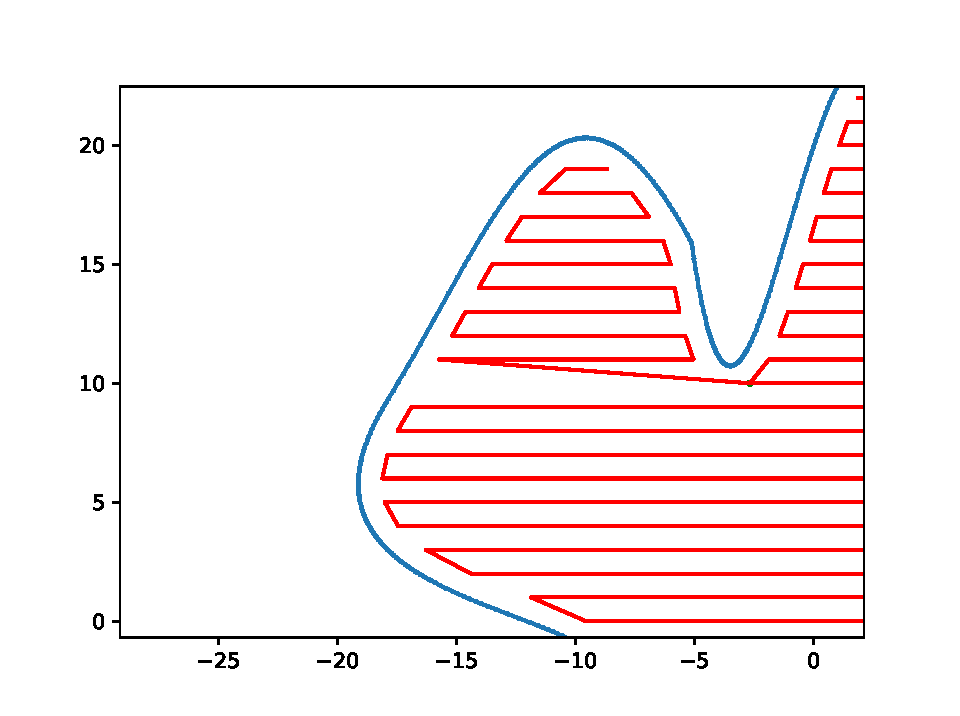
\includegraphics[width=7cm]{zigzag detail 1mm}
    \caption{\CJK{UTF8}{gbsn}{zigzag hatching detail with $0.1mm$ accuracy}}
    \caption{\CJK{UTF8}{gbsn}{zigzag hatching detail
            with $1mm$ accuracy}}
\end{figure}

The above pictures show the details of the same part under two precisions. Under low precision, due to the order of the points, at the boundary of the partition, the points on the left are directly connected to the points on the right not in the same row, resulting in sharp angles. But with high precision, this kind of flaw is reduced and hidden in the zigzag curve, which is difficult to be found and can be ignored.

\subsubsection{The contour parallel hatch}


\begin{figure}[!ht]
    \centering
    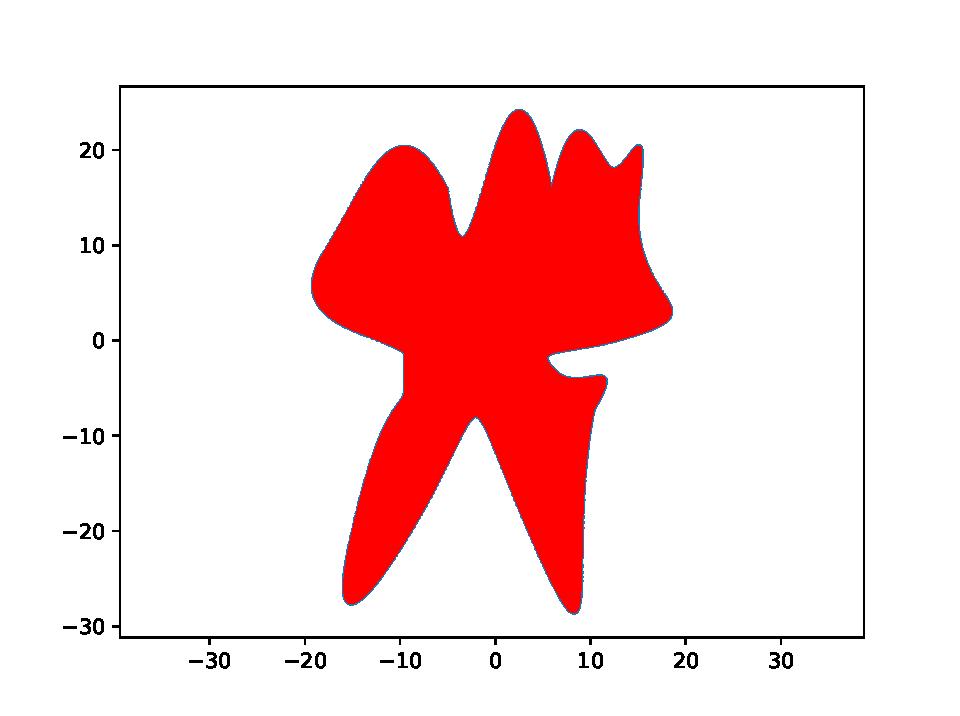
\includegraphics[width=7cm]{contour0.1mm} \quad 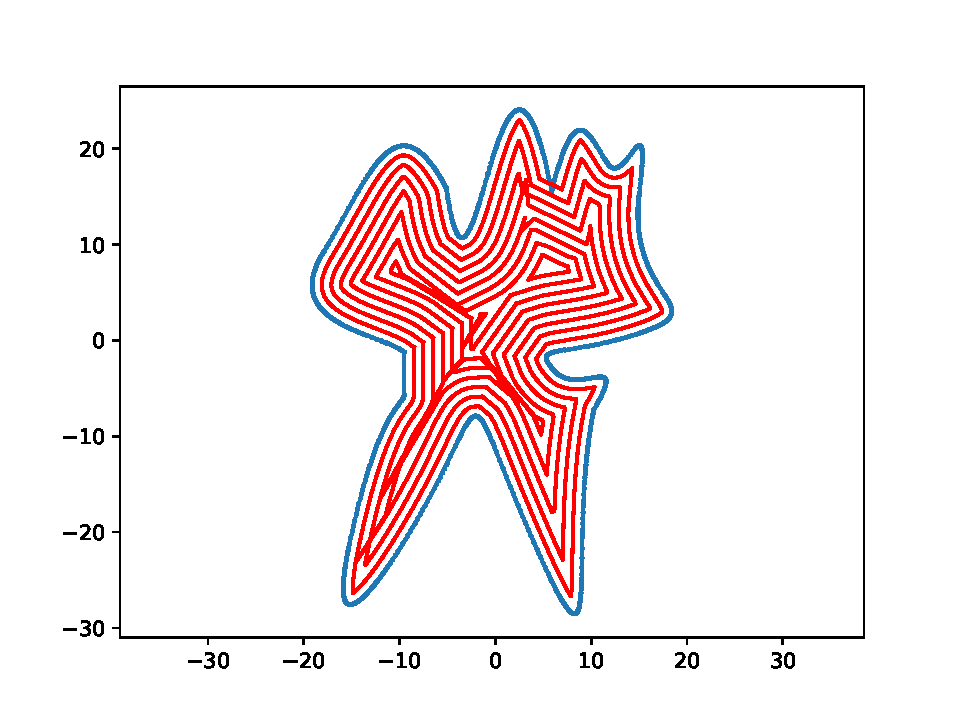
\includegraphics[width=7cm]{contour1mm}
    \caption{\CJK{UTF8}{gbsn}{contour parallel hatching with $0.1mm$ accuracy}}
    \caption{\CJK{UTF8}{gbsn}{contour parallel hatching with $1mm$ accuracy}}
\end{figure}

When the accuracy is $1mm$, the total length of the curve is $985.26mm$, the number of circles is $11$, and the average elapsed time is $(2.91\times 10^4\pm 200)$ mm. When the accuracy is $0.1mm$, the total length of the curve is $10060.39mm$, the number of circles is $129$, and the average elapsed time is $(6.25\times 10^5\pm 2000)$ mm. The time-consuming ratio in the two cases is $21.48$.


\begin{figure}[!ht]
    \centering
    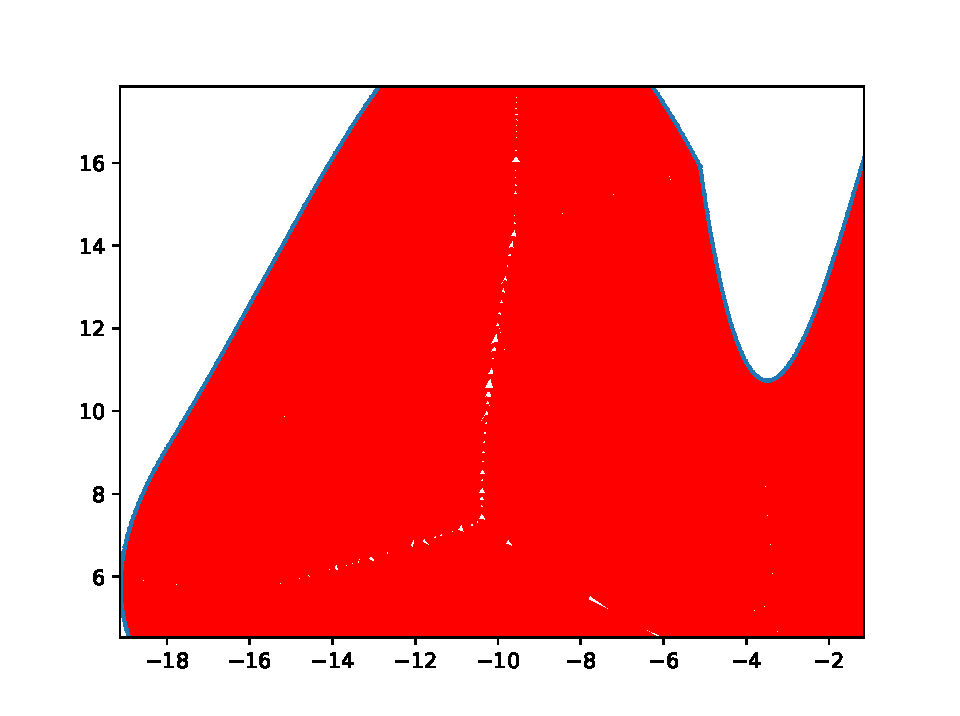
\includegraphics[width=7cm]{contour detail 0.1mm} \quad 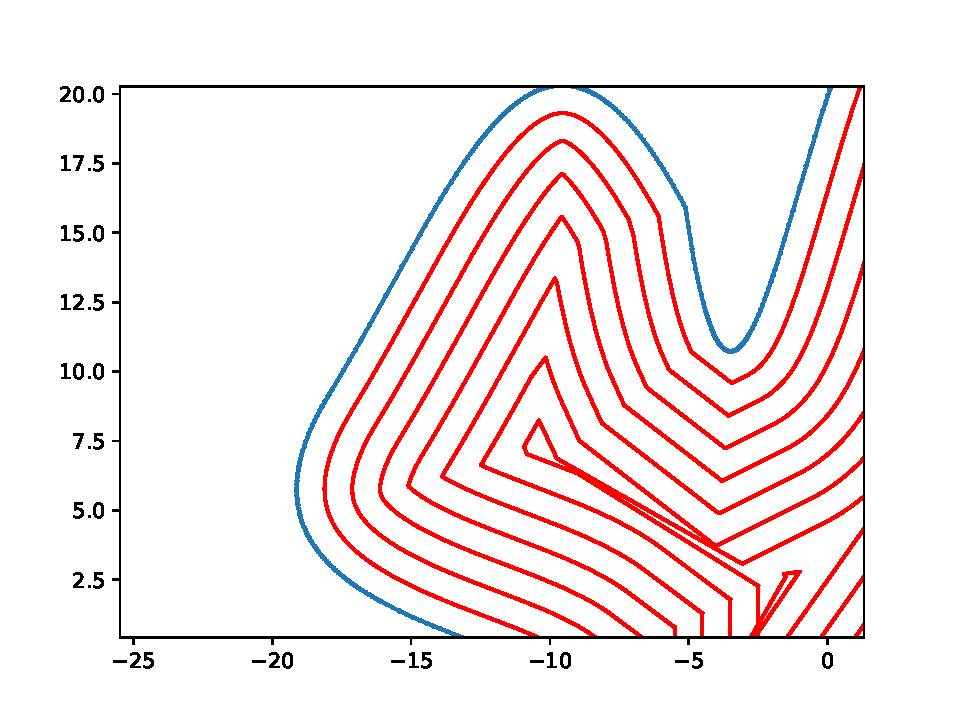
\includegraphics[width=7cm]{contour detail 1mm}
    \caption{\CJK{UTF8}{gbsn}{contour parallel detail hatching with $0.1mm$ accuracy}}
    \caption{\CJK{UTF8}{gbsn}{contour parallel detail hatching with $1mm$ accuracy}}
\end{figure}

Reducing the same accuracy, the algorithm takes significantly longer time. At low precision, some lines overlap. Due to the limitation of the initial data volume, we must add a certain number of points to ensure the curve is closed, which leads to the generation of blanks at the smaller radius of curvature. This effect is more obvious under high precision.

\subsubsection{Comparison of two hatch methods}

For zigzag hatch, the advantage is that the coordinates of the original geometric figure are rounded, and the zigzag line of the entire figure can be generated only through the data of the boundary. Because of the rounding operation, the algorithm does not need to meet other requirements for the relative position between the points in the original data, and only needs to judge and process according to the ordinate of the point. For the internal main part of the graph, the algorithm does not need to be processed. In the actual laser marking process, most of the time the laser marking machine only performs one-dimensional movement and only needs a servo motor to work.


Comparing contour hatching with glyph hatching, its biggest feature is the huge amount of data and the huge computational workload. This is because the point data on each contour line needs to be generated from the point data on the previous contour line. Taking the data in this question as an example, under the same 0.1mm accuracy condition, the zigzag hatching algorithm only produced 1816 points, while the contour hatching algorithm produced 78578 points. Due to the increase in the number of points and more conditions for the contour line to be judged, the calculation amount of the contour line algorithm will be very large. The most direct manifestation is the extension of calculation time. At 0.1mm accuracy, the contour algorithm takes more than 10 minutes, while the zigzag algorithm only takes about 7 seconds. However, it is precisely because of more data that the accuracy of the contour algorithm on the boundary will be higher in the same situation. For example, in the zigzag algorithm, two adjacent horizontal lines are separated by one accuracy unit, but the abscissas of their endpoints on the same side may be very different, so the actual distance between the two points will be very far. The distance between the points on the boundary of the contour algorithm is always related to the initial data. As long as the distance between two adjacent points of the initial data is close enough, the distance between the points produced will not become particularly far.


\subsection{hatch of multiply-connected domain}

Due to the limitation of time and calculation conditions, we have not been able to complete the hatching of the two ways of multiply-connected domain. Only our ideas for solving this problem are given here.

\subsubsection{The direction parallel hatch}

Like the single connected domain, the multiply-connected domain should also be divided into areas in the zigzag hatch. For example, there is a contour line C0, and other contour lines C1, C2... we should take the extreme value of each contour line in the vertical axis direction, and make a horizontal line through each extreme value point. If the number of intersection points is the same on its both sides, the point is confirmed as the starting point of a dividing line, and the first focus of the front of the sequence is the end of the dividing line. Just like the single connected domain, we can get several regions, and then fill these regions with zigzag lines.


\subsubsection{The contour parallel hatch}

In the multiply-connected domain, in addition to the segmentation of contours, there is also the merging of contours. When the same-level inner shrinking lines from different contours are close, they need to be merged into a contour line in a certain order. It means that two interrupted points are connected to each other, and connect one of the contour lines to the end, and then continue to fill in according to the method of single connected domain.

\section{Conclusions}

\subsection{Conclusions of the problem}

Both algorithms have basically realized the automation of path planning, and in most cases they have a high degree of satisfaction with accuracy. However, for some special and extreme situations, the program cannot be accurately identified and processed automatically. The user needs to manually set the boundary condition parameters based on experience and actual conditions.


Comparing the two algorithms, we an see that under the same accuracy conditions, the total path length calculated by the zigzag algorithm and the contour algorithm is basically the same, but the total data volume of the zigzag hatch is much less. With the same computer, the running time of the program is much shorter. In the actual laser marking process, with the zigzag hatch, the movement of the marking machine will be much easier, so its advantages are more obvious. But this does not mean that the contour parallel hatch has no advantages. Under the same accuracy conditions, the contour algorithm will be more accurate in processing the graphics boundary.


\subsection{Methods used in our algorithm}

\subsubsection{The direction parallel hatch}

The zigzag hatch is embodied in our algorithm as a problem of reordering the data points. For the data points generated after indentation, we partition them according to the geometric shapes they form, and order the points on each area according to the ordinate. By connecting the data points we ordered we get several sets of zigzag curves.

\subsubsection{The contour parallel hatch}

Here we have adopted a method similar to a binary tree. Through a series of calculations on the original data points, a new set of data points is obtained; the same calculation is performed on the new data points to obtain the next set of data points. There is a correspondence between the data points in each group. But unlike the binary tree method, this method has a one-to-one correspondence between the old and new data points. Therefore, some areas will produce some points that destroy the shape of the figure, and our algorithm will delete them based on the geometric properties of the figure formed by these points.

\subsection{The advantages and disadvantages of the algorithms}

\subsubsection{The direction parallel hatch}

Advantage:


1) Partition processing can ensure that each independent area can generate a single zigzag line.


2) The representation of variables can be simplified, and in most cases. Floating-point operations can be turned into integer operations.


3) When the distance between two points is too large, points with integer multiples of precision can be automatically added to ensure that the zigzag line can cover the area completely.


4) The amount of data is small. The calculation complexity is determined by the geometric size of the figure.


Disadvantages:


1) The problem of boundary conditions. The endpoints of the independent partitions may overlap, and unnecessary connecting lines may be generated during the running of the program.


2) Multiple independent areas will increase the no-load running time of the laser marking machine during actual operation.


\subsubsection{The contour parallel hatch}


advantage:


1) We use vector coordinates to transform. The way to generate new points is relatively simple.


2)Deleting at a position that is too small in most cases not only ensures that the graph will not change suddenly, but also reduces a certain amount of calculation.


Disadvantages:


1) It will generate a lot of data. Each contour line will generate a new set of point coordinate data.


2) The judgment condition requires a lot of calculation. To ensure as far as possible that the images will not appear cross and overlap errors, the program needs to calculate a large amount of distance data. These calculations almost use the coordinate data of all points, but most of the calculation results have nothing to do with the final output results.

\subsection{Applications of our algorithm}

The algorithm we proposed realizes the filling of two-dimensional closed curve polygons through zigzag hatching and contour parallel hatching. It is expected to be used in laser marking after further optimization. In addition, we will increase the dimensionality of the algorithm in future work to enable it to fill the three-dimensional closed space. This can open exciting perspectives for 3d printing, laser engraving, etc.

\section{Future Work}
\subsection{Ideas to solve existing problems}
Zigzag, as the most common hatching method at present, has many sharp turns. For shapes with complex borders or hollow, this disadvantage will be very obvious.The contour parallel algorithm can avoid too many sharp turns, but it leads to more contours and the contours are not connected. For the problems of these two hatching methods, we can use the Fermat spiral filling to solve it. The Fermat spiral consists of two intertwined sub-helices, one inward and the other outward. The Fermat spiral has three advantages:
\cite{2}


1) Similar to the contour parallel hatch, the Fermat spiral only has a sharp turn at the center.


2) Some Fermat spirals can continuously fill the 2D area; traditional spirals are either inward or outward, and Fermat spirals are both inward and outward, and can meet at the boundary.


3) To facilitate the connection between the spirals, the start and end nodes of the Fermat spiral can be selected arbitrarily at the boundary.
\subsection{Optimization of performance and efficiency}
\subsubsection{Reducing the idling of the robotic arm}
In actual industrial applications, in addition to the running time of the algorithm, we must consider another time cost, the efficiency of the robot's movement. For the zigzag hatch, according to the complexity of the graphics, we have to partition them. This results in a certain distance between the start and end of each curve. It takes a certain amount of time for the robot arm to move between them. In order to reduce this waste, we need to make a more reasonable design for the partition and the angle between the parallel line and the x-axis. In the same way, there will be multiple converging centers in contour hatching. Reducing the number of converging centers as much as possible means reducing the blank movement time of the robotic arm.

\subsubsection{Reducing the amount of data}
In the actual laser marking process, the original image often contains a large number of data points. To delete redundant or isolated data points can shorten the running time of the program.
\subsubsection{Program optimization\cite{1}}

1)Algorithm optimization:
An excellent algorithm can reduce the complexity of the algorithm by several orders of magnitude, and its average time-consuming is generally less than other algorithms with high complexity
There is another situation where the algorithm itself is relatively complicated, its time complexity is difficult to reduce, and its efficiency does not meet the requirements. The measures that can be taken are: maintaining the effect of the algorithm to improve efficiency, and discarding part of the effect in exchange for a certain efficiency.


2)Code optimization:


a. Avoid multiplication (division) and redundant calculations inside the loop


b. Avoid too many dependencies and jumps inside the loop


c. Convert floating-point operations to integer operations


d. Exchange space for time


e. Pre-allocated memory


3)Instruction optimization
Instruction optimization generally uses a specific instruction set to quickly implement certain operations. Another core idea of instruction optimization is packed operations.

\subsubsection{Multi-Progress operation}
Due to the limitation of single-Progress, our code can only run in a single process. However, we found that after partitioning, the iteration of each region, the correspondence between points, and the detection of each point are relatively independent, which makes it possible for some programs to run in multiple process. Through multi-Progress processing, we can greatly reduce the running time of the program, thereby improving its performance.




%参考文献
\begin{thebibliography}{9}%宽度9
    \bibitem{1} \CJK{UTF8}{gbsn}{浅谈程序优化} \url{https://www.cnblogs.com/jcchen1987/p/4362879.html}
    \bibitem{2} \CJK{UTF8}{gbsn}{3D打印路径填充算法} \url{https://blog.csdn.net/weixin_33769207/article/details/93196133?utm_source=app}
\end{thebibliography}

\newpage
%附录

\section{Appendix}
\begin{lstlisting}[language=Python,caption={The python Source code of contour parallel hatch}]
  import matplotlib.pyplot as plt 
  import numpy as np
  from numpy.core.fromnumeric import argmax, argmin
  import pandas as pd
  import math
  import time
  
  start = time.thread_time()
  
  data = np.array(pd.read_csv(".\code\graph1.csv", header=2))   
  d = -0.1  # -0.1 or 1
  plt.axis("equal")
  plt.plot(data[:, 0], data[:, 1], '-o', markersize=1)
  dots = 0
  
  
  def findex(data, i):   
      if (data[i, 1] >= data[i-1, 1] and data[i, 1] > data[i+1, 1]) or (data[i, 1] <= data[i-1, 1] and data[i, 1] < data[i+1, 1]):
          return(1)
      else:
          return(0)
  
  
  def unit(v):   
      return(v/np.linalg.norm(v))
  
  
  def angle(v):   
      return(math.atan2(v[1], v[0]))
  
  
  def inangle(v1, v2):   
      return(math.acos(np.dot(v1, np.transpose(v2)) / (np.linalg.norm(v1)*np.linalg.norm(v2))))
  
  
  def drawborder(data):   
      data = np.insert(data, data.shape[0], values=data[1, :], axis=0)
      data = np.insert(data, 0, values=data[data.shape[0]-3, :], axis=0)
      temp = np.array([0, 0])
      times = data.shape[0]-2
      i = 0
      while i < times:
          k = 0
          v1 = data[i+1, :]-data[i, :]
          v2 = data[i+2, :]-data[i+1, :]
          u = d/(math.sin(inangle(v1, v2)))
          if (angle(v2) > angle(v1) and not(angle(v2) > math.pi/2 and angle(v1) < -math.pi/2)) or (angle(v2) < -math.pi/2 and angle(v1) > math.pi/2):
              new = data[i+1, :]+(unit(v2)-unit(v1))*u
          else:
              new = data[i+1, :]-(unit(v2)-unit(v1))*u
          for j in range(0, data.shape[0]-2):
              if np.linalg.norm(new-data[j, :]) < abs(d)*0.999:
                  k = 1
                  break
          if k == 0:
              temp = np.row_stack((temp, new))
          i += 1
      temp = np.delete(temp, 0, axis=0)
       plt.plot(temp[:, 0], temp[:, 1], '-o', color='y', markersize=2)
      return(temp)
  
  
  def getint(data):   
      temp = new = np.array([0, 0.])
      for i in range(data.shape[0]-1):
          x1 = data[i, 0]
          y1 = data[i, 1]
          x2 = data[i+1, 0]
          y2 = data[i+1, 1]
          k = (y2-y1)/(x2-x1)   
          if y1//abs(d) < y2//abs(d):
              for j in range(1, math.floor(y2//abs(d)-y1//abs(d)+1)):
                  new[1] = round((y1//abs(d)+j)*abs(d), 1)
                  new[0] = (new[1]-y1)/k+x1
                  temp = np.row_stack((temp, new))
          else:
              if y1//abs(d) > y2//abs(d):
                  for j in range(0, math.floor(y1//abs(d)-y2//abs(d))):
                      new[1] = round((y1//abs(d)-j)*abs(d), 1)
                      new[0] = (new[1]-y1)/k+x1
                      temp = np.row_stack((temp, new))
      temp = np.delete(temp, 0, axis=0)
       plt.plot(temp[:, 0], temp[:, 1], '-o', color='g', markersize=2)
      return(temp)
  
  
  def getdline(data):   
      temp = 0
      dline = np.array([0, 0, 0])
      for i in range(1, data.shape[0]-2):
          k = 0
          if findex(data, i) == 1:
              for j in range(data.shape[0]*2//3):
                  if j+i >= data.shape[0]-1:
                      l = j-data.shape[0]
                  else:
                      l = j
                  if data[i+l+1, 1] == data[i, 1]:
                      temp = i+l+1
                      if data[i+l+1, 0] > data[i, 0]:
                          k += 2
                      else:
                          k += 1
                      break
              for j in range(data.shape[0]*2//3):
                  if data[i-j-2, 1] == data[i, 1]:
                      if data[i-j-2, 0] > data[i, 0]:
                          k += 2
                      else:
                          k += 1
                      break
              if k == 3:
                  dline = np.array([data[i, 1], i, temp])
                  print(dline)
                  dots = np.array([data[math.floor(dline[1]), :],
                                   data[math.floor(dline[2]), :]])
                  plt.plot(dots[:, 0], dots[:, 1], '--o',
                           color='g', markersize=2)
                  return(dline)
      print(dline)
      return(dline)
  
  
  def divide(data):   
      i = 0
      while True:
          dline = getdline(data[i])
          if dline[1] == 0 and dline[2] == 0:
              i += 1
          else:
              temp = data[i]
              data.append(temp[math.floor(dline[1]): math.floor(dline[2])+1, :])
              temp1 = temp[0:math.floor(dline[1])+1, :]
              temp2 = temp[math.floor(dline[2]):temp.shape[0], :]
              data[i] = np.row_stack((temp1, temp2))
              continue
          if i == len(data):
              break
      return(data)
  
  
  def writecsv(data):
      for i in range(len(data)):
          area = data[i]
          dataframe = pd.DataFrame(data={'x': area[:, 0], 'y': area[:, 1]})
          dataframe.to_csv(f".\code\\area{i}.csv",
                           index=False, mode='w', sep=',')
      pass
  
  
  def drawline(data):   
      global dots
      length = 0   
      times = 0   
      for i in range(len(data)):
          line = np.array([0, 0])
          area = data[i]
          maxy = round(max(area[:, 1]), 1)
          miny = round(min(area[:, 1]), 1)
          j = miny
          while j <= maxy:
              index = (np.where(area == j))[0]
              temp = area[index, 0]
              if round(j/abs(d)) % 2:
                  line = np.row_stack((line, [j, min(temp)]))
                  temp = np.delete(temp, argmin(temp))
                  line = np.row_stack((line, [j, min(temp)]))
              else:
                  line = np.row_stack((line, [j, max(temp)]))
                  temp = np.delete(temp, argmax(temp))
                  line = np.row_stack((line, [j, max(temp)]))
              j = round(j + abs(d), 1)
          line = np.delete(line, 0, axis=0)
          plt.plot(line[:, 1], line[:, 0], '-', color='r')
          times = times+int(line.shape[0]/2)
          for j in range(line.shape[0]-1):
              length = length + \
                  math.sqrt((line[j+1, 0]-line[j, 0])**2 +
                            (line[j+1, 1]-line[j, 1])**2)
              dots += 1
          i += 1
      return([length, times])
  
  
  data = drawborder(data)
  data = getint(data)
  data = list([data])
  data = divide(data)
  writecsv(data)
  data = drawline(data)
  
  end = time.thread_time()
  print('Length of curve:         %s mm' % data[0])
  print('Number of parallel line: %s' % data[1])
  print('Number of dots: %s' % dots)
  print('Running time:            %s Seconds' % (end-start))
  
  plt.show()
  
\end{lstlisting}
\begin{lstlisting}[language=Python,caption={The python source code of zigzag hatch}]
  import matplotlib.pyplot as plt
  import numpy as np
  import pandas as pd
  import math
  import time
  
  start = time.thread_time()
  
  data0 = np.array(pd.read_csv(".\code\graph1.csv", header=2))
  data = data0  
  d = -0.1  # -0.1 or -1
  plt.axis("equal")
  plt.plot(data[:, 0], data[:, 1], '-o', markersize=1)
  dots = 0
  
  
  def unit(v):  
      return(v/np.linalg.norm(v))
  
  
  def angle(v):  
      return(math.atan2(v[1], v[0]))
  
  
  def inangle(v1, v2):  
      return(math.acos(round(np.dot(v1, np.transpose(v2)) / (np.linalg.norm(v1)*np.linalg.norm(v2)), 9)))
  
  
  def draw(data):  
      global dots
      data = np.insert(data, data.shape[0], values=data[1, :], axis=0)
      data = np.insert(data, 0, values=data[data.shape[0]-3, :], axis=0)
      temp = np.array([0, 0])
      i = 0
      while i < data.shape[0]-2:
          v1 = data[i+1, :]-data[i, :]
          v2 = data[i+2, :]-data[i+1, :]
          if 0 < inangle(v1, v2) < math.pi*0.9:  
              u = d/(math.sin(inangle(v1, v2)))
              if (angle(v2) > angle(v1) and not(angle(v2) > math.pi/2 and angle(v1) < -math.pi/2)) or (angle(v2) < -math.pi/2 and angle(v1) > math.pi/2):
                  new = data[i+1, :]+(unit(v2)-unit(v1))*u
              else:
                  new = data[i+1, :]-(unit(v2)-unit(v1))*u
          else:
              if inangle(v1, v2) == 0:  
                  if angle(v1) > 0:
                      new = data[i+1, :] + unit([v1[1], -v1[0]])*abs(d)
                  else:
                      new = data[i+1, :] - unit([-v1[1], v1[0]])*abs(d)
              else:  
                  i += 1
                  continue
          i += 1
          temp = np.row_stack((temp, new))
          dots += 1
      temp = np.delete(temp, 0, axis=0)
      temp = iflong(temp)  
      temp = ifcross(temp)  
      temp = ifwide(temp, data)  
      plt.plot(temp[:, 0], temp[:, 1], '-', color='r')
      return(temp)
  
  
  def iflong(data):  
      i = 0
      while i < data.shape[0]-1:  
          if np.linalg.norm(data[i+1, :]-data[i, :]) > 2*abs(d):  
              new = np.array([(data[i+1, 0]+data[i, 0])/2,
                              (data[i+1, 1]+data[i, 1])/2])
              data = np.insert(data, i+1, new,  axis=0)
              continue
          else:
              i = i+1
      return(data)
  
  
  def ifwide(data, last):  
      i = 0
      while i < data.shape[0]:  
          j = 0
          while j < last.shape[0]:  
              if i >= data.shape[0]:
                  break
              if np.linalg.norm(data[i, :]-last[j, :]) < abs(d)*0.999:  
                  data = np.delete(data, i, axis=0)
                  if j > 20:
                      j -= 20
                  else:
                      j = 0
              else:
                  j += 1
          i += 1
      return(data)
  
  
  def ifcross(data):  
      i = 0
      while i < data.shape[0]-3:  
          v1 = data[i+1, :]-data[i, :]
          v2 = data[i+2, :]-data[i+1, :]
          v3 = data[i+3, :]-data[i+2, :]
          if inangle(v1, v2)+inangle(v2, v3) > math.pi:  
              data = np.delete(data, [i+1, i+2], axis=0)
          else:
              i += 1
      return(data)
  
  
  def ifdivide(data):  
      for i in range(data.shape[0]-2):
          for j in range(i, data.shape[0]-2):
              x1 = data[i, 0]
              y1 = data[i, 1]
              x2 = data[j, 0]
              y2 = data[j, 1]
              if 0 < math.sqrt((x2-x1)**2+(y2-y1)**2) < abs(d) and j-i > 3:  
                  v1 = data[i+2, :]-data[i, :]
                  v2 = data[j+2, :]-data[j, :]
                  if abs(angle(v1)-angle(v2)) > math.pi/2:
                      return(np.array([i, j]))
      return(np.array([0, 0]))
  
  
  def drawline(data):  
      length = 0
      times = 0
      while True:
          temp = data[-1]
          if data[0].shape[0] < 10:
              break
          if temp.shape[0] < 10:
              del data[len(data)-1]
              print('-')
              continue
          index = ifdivide(temp)  
          if index[0] == 0 and index[1] == 0:
              data[-1] = draw(temp)
              print(times)
              times += 1
              for j in range(data[-1].shape[0]-1):
                  length = length + \
                      math.sqrt((data[-1][j+1, 0]-data[-1][j, 0])**2 +
                                (data[-1][j+1, 1]-data[-1][j, 1])**2)
               plt.plot(data0[:, 0], data0[:, 1], '-o', color='b', markersize=1)
               plt.show()
               plt.axis("equal")
          else:
              data.append(temp[math.floor(index[0])+1: math.floor(index[1]), :])
              data[-1] = np.row_stack((data[-1], data[-1][0:1, :]))
              temp1 = temp[0:math.floor(index[0])+1, :]
              temp2 = temp[math.floor(index[1]):temp.shape[0], :]
              data[-2] = np.row_stack((temp1, temp2))
      return([length, times])
  
  
  data = list([data])
  data = drawline(data)
  
  end = time.thread_time()
  print('Length of curve: %s mm' % data[0])
  print('Number of turns: %s' % data[1])
  print('Number of dots: %s' % dots)
  print('Running time:    %s Seconds' % (end-start))
  
  plt.show()
  
\end{lstlisting}


\end{document}